\documentclass[15pt,a4paper]{report}
\usepackage[utf8]{vietnam}
\usepackage{amsmath}
\usepackage{amsfonts}
\usepackage{hyperref}
\usepackage{amsmath}
\usepackage{graphicx}
\usepackage{hyperref}
\usepackage{float} % Cần thiết cho tùy chọn [H]
\usepackage[utf8]{vietnam}
\usepackage{amsmath}
\usepackage{amsfonts}
\usepackage{amssymb}
\usepackage{graphicx}
\usepackage[left=1cm,right=1cm,top=1.5cm,bottom=1.5cm]{geometry}
\usepackage{blindtext}
\usepackage{titlesec}
\usepackage{graphicx}
\usepackage{multicol}
\usepackage{url}
\usepackage{matlab-prettifier}
\usepackage{caption}
\usepackage{arydshln}
\usepackage{mdframed}
\usepackage{amsthm}
\usepackage{listings}
\usepackage{xcolor}
\lstset{ 
	language=R,                % Ngôn ngữ
	basicstyle=\ttfamily\footnotesize, % Phông chữ
	%keywordstyle=\color{blue}, % Màu cho từ khóa
	commentstyle=\color{green!50!black}, % Màu cho chú thích
	stringstyle=\color{red},   % Màu cho chuỗi
	showstringspaces=false,    % Không hiển thị khoảng trắng trong chuỗi
	numbers=left,              % Hiển thị số dòng bên trái
	numberstyle=\tiny\color{gray}, % Phong chữ cho số dòng
	frame=single,              % Kẻ khung cho đoạn mã
	breaklines=true            % Tự động xuống dòng
}
\usepackage{graphicx}
\usepackage{pgfplots}
\fontsize{20pt}{15pt}
\usepgfplotslibrary{fillbetween}
\usetikzlibrary{patterns}


%%%%%%% code setup
\usepackage{listings}
\usepackage{caption}
\usepackage{xcolor}

% Không caption đánh số
\DeclareCaptionOption{lstlisting}{caption=false}{} 
\captionsetup[lstlisting]{labelformat=empty, position=bottom}

% (Tuỳ chọn) Màu nền nhẹ
\definecolor{mybg}{rgb}{0.94,0.94,0.94}

% Định nghĩa R
\lstdefinelanguage{R}{
	basicstyle=\ttfamily\small,
	keepspaces=true,
	showstringspaces=false,
	columns=fullflexible,
	upquote=true
}

% Định nghĩa Python
\lstdefinelanguage{Python}{
	basicstyle=\ttfamily\small,
	keepspaces=true,
	showstringspaces=false,
	columns=fullflexible,
	upquote=true
}

% Tắt hoàn toàn lề trái
\setlength{\parindent}{0pt}    % Không thụt lề đoạn văn
\setlength{\leftskip}{0pt}     % Không dịch trái toàn đoạn
\lstset{
	backgroundcolor=\color{mybg},
	breaklines=true,
	frame=none,
	numbers=none,
	xleftmargin=0pt,
	xrightmargin=0pt
}

%%%%%% end code setup

\begin{document}
\[
	\boxed{\huge \textbf{House Rent Analysis}}
\]
\section*{Data Preparation}
I have introduced the dataset \lstinline[language=R]|munichrent03| which is integrated in the R package \lstinline[language=R]|LinRegInteractive|, available at \textbf{\href{https://github.com/taitran0102/rent-analysis/blob/main/README.md}{README.md}} file. Therefore, I can simply load this dataset to begin the subsequent steps of the analysis.
\begin{lstlisting}[language=R]
library(LinRegInteractive)
data(munichrent03)
data <- munichrent03 
\end{lstlisting}
I began by examining the variable types to understand the structure of the dataset. 
\begin{lstlisting}[language=R]
> str(data)
'data.frame':	2053 obs. of  12 variables:
$ rent     : num  741 716 528 554 698 ...
$ rentsqm  : num  10.9 11.01 8.38 8.52 6.98 ...
$ area     : int  68 65 63 65 100 81 55 79 52 77 ...
$ rooms    : int  2 2 3 3 4 4 2 3 1 3 ...
$ yearc    : num  1918 1995 1918 1983 1995 ...
$ bathextra: Factor w/ 2 levels "no","yes": 1 1 1 2 2 1 2 1 1 1 ...
$ bathtile : Factor w/ 2 levels "yes","no": 1 1 1 1 1 1 1 1 1 1 ...
$ cheating : Factor w/ 2 levels "yes","no": 1 1 1 1 1 1 1 1 1 1 ...
$ district : Factor w/ 25 levels "All-Umenz","Alt-Le",..: 10 10 10 17 17 17 21 21 21 21 ...
$ location : Ord.factor w/ 3 levels "normal"<"good"<..: 2 2 2 1 2 1 1 1 1 1 ...
$ upkitchen: Factor w/ 2 levels "no","yes": 1 1 1 1 2 1 1 1 1 1 ...
$ wwater   : Factor w/ 2 levels "yes","no": 1 1 1 1 1 1 1 1 1 1 ...
> names(data)
'rent''rentsqm''area''rooms''yearc''bathextra''bathtile''cheating''district''location''upkitchen''wwater'
\end{lstlisting}
After that, I reviewed the distributions, value ranges, and identified any potential missing values.
\begin{lstlisting}[language=R]
> summary(data)
      rent            rentsqm            area           rooms      
Min.   :  77.31   Min.   : 1.470   Min.   : 17.0   Min.   :1.000  
1st Qu.: 389.95   1st Qu.: 6.800   1st Qu.: 53.0   1st Qu.:2.000  
Median : 534.30   Median : 8.470   Median : 67.0   Median :3.000  
Mean   : 570.09   Mean   : 8.394   Mean   : 69.6   Mean   :2.598  
3rd Qu.: 700.48   3rd Qu.:10.090   3rd Qu.: 83.0   3rd Qu.:3.000  
Max.   :1789.55   Max.   :20.090   Max.   :185.0   Max.   :6.000  

yearc      bathextra  bathtile   cheating        district      location   
Min.   :1918   no :1862   yes:1673   yes:1878   Neuh-Nymp: 177   normal:1205  
1st Qu.:1948   yes: 191   no : 380   no : 175   Lud-Isar : 161   good  : 803  
Median :1960                                    Au-Haid  : 139   top   :  45  
Mean   :1958                                    SchwWest : 137                
3rd Qu.:1973                                    Maxvor   : 132                
Max.   :2001                                    Laim     : 117                
(Other)  :1190                
upkitchen  wwater    
no :1903   yes:1981  
yes: 150   no :  72  

\end{lstlisting}
Note that the variables \lstinline[language=R]|rentsqm, rent| and \lstinline[language=R]|area| are related by the equation: \lstinline[language=R]|rent| = \lstinline[language=R]|rentsqm| $\times$ \lstinline[language=R]|area|. For example, at row 100, we have:

\begin{lstlisting}[language=R]
> round(data$rent[100]/data$area[100],2)  #compute rentsqm
11.3
> data$rentsqm[100]
11.3
\end{lstlisting}
Since \lstinline[language=R]|rentsqm| is a derived variable, I chose to exclude it and instead focus on total \lstinline[language=R]|rent|, which may better capture the underlying relationships with other features.
\begin{lstlisting}[language=R]
> data$rentsqm <- NULL
\end{lstlisting}
\section*{Exploratory Data Analysis}
Subsequently, I conducted an Exploratory Data Analysis (EDA) to gain initial insights into the dataset. A few key findings from this phase include:
\begin{itemize}
	\item The 7 districts with the largest number of houses
	\begin{lstlisting}[language=R]
Neuh-Nymp  Lud-Isar   Au-Haid  SchwWest    Maxvor      Laim   Ram-Per 
177        161        139       137        132         117       115 
	\end{lstlisting}
	\item The 7 districts with the highest number of houses where the location is classified as either “top” or “good”:
		\begin{lstlisting}[language=R]
Maxvor   Neuh-Nymp    Lud-Isar    SchwWest     Au-Haid Schwab-Frei    Trud-Rie 
118         116          97          96          81          50          37 
	\end{lstlisting}
	\item The proportion of houses equipped with each feature:
	\begin{lstlisting}[language=R]
    Feature Count Percent
1 bathextra   191     9.3
2  bathtile  1673    81.5
3  cheating  1878    91.5
4 upkitchen   150     7.3
5    wwater  1981    96.5
	\end{lstlisting}
	\item The distribution of the numerical variables in the dataset
	\begin{figure}[H]
		\centering 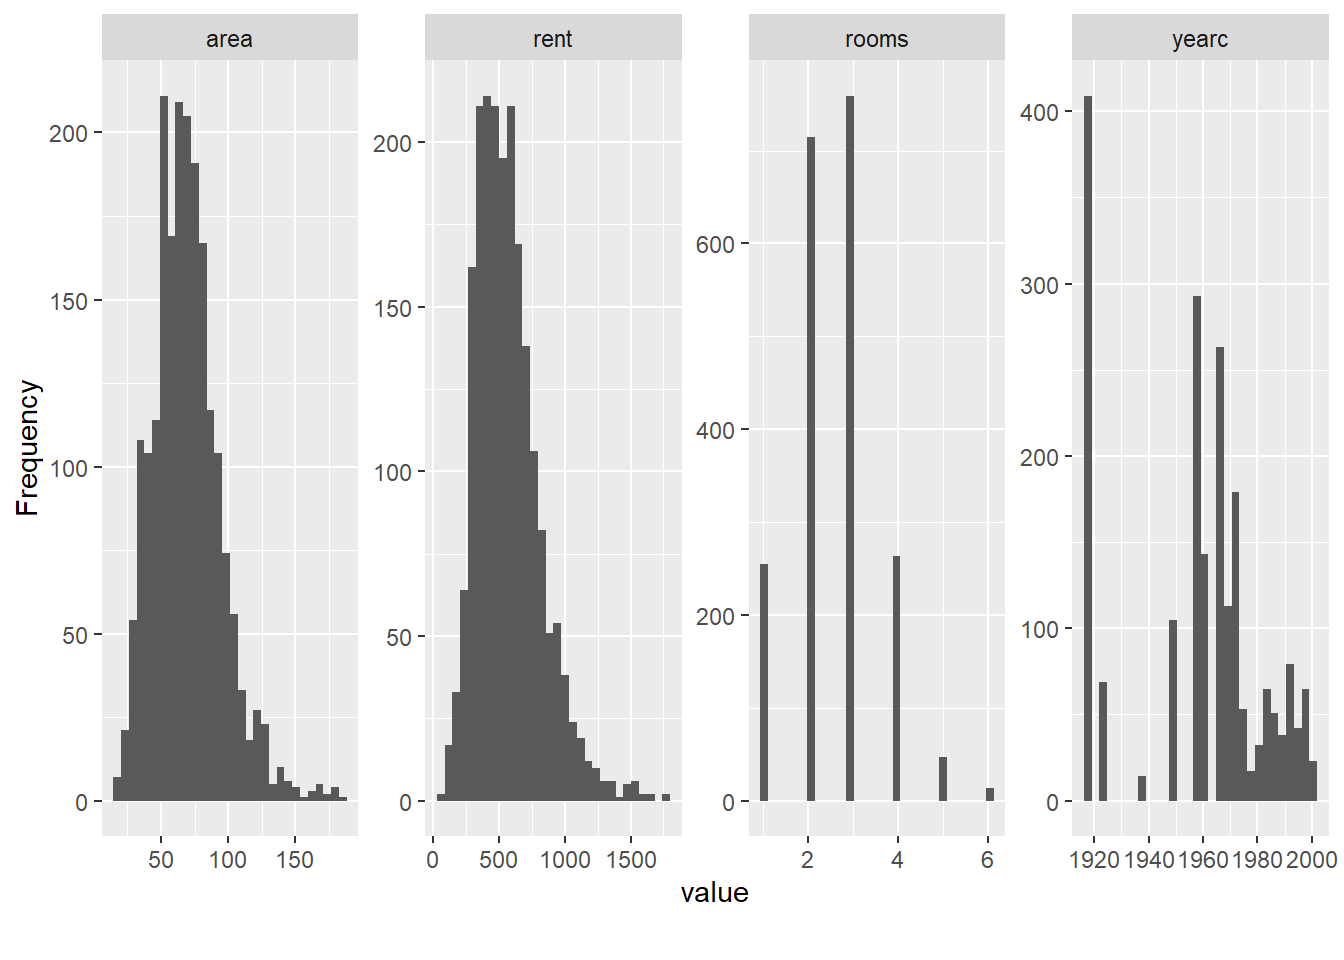
\includegraphics[width=\textwidth]{unnamed-chunk-10-1.png}
	\end{figure}
	\item The variable \lstinline[language=R]|yearc| represents discrete individual years, and the number of rooms(\lstinline[language=R]|room|)ranges only from 1 to 6.
		\begin{lstlisting}[language=R]
> table(data$room) #Count for each number of room

1   2   3   4   5   6 
255 715 759 263  47  14 
> table(data$yearc) #Count for each year

1918   1924   1939   1948   1957 1957.5   1960   1966   1967   1968 
409     69     14    105    225     68    143    228     35     23 
1969   1970   1971   1972   1973   1974   1975   1976   1977   1978 
44     46     35     89     55     30     16      7      6      5 
1979   1980   1981   1982   1983   1984   1985   1986   1987   1988 
6     17     15      8     40     17     20     11     20     13 
1989   1990   1991   1992   1993   1994   1995   1996   1997   1998 
15     10     14     24     41     13      9     20     12     14 
1998.5   1999   2000   2001 
32      7     18      5 
	\end{lstlisting}
\end{itemize}
\section*{Graphical Model Learning}
\subsubsection*{More Data Preparation}
To learn a model from the data, some additional preprocessing steps are required. From the earlier exploration, I observed that the dataset contains many categorical variables, and only two variables, namely rent and area, are truly continuous. 

A Directed Graphical Model can be used to model data under two common distributional assumptions:
\begin{itemize}
	\item Multinomial (each variable is categorical)
	\item Multivariate Normal
\end{itemize}

Since the dataset contains mostly categorical variables, I decided to model the data assuming a Multinomial distribution. Therefore, several variables needed to be transformed accordingly. Below is a summary of the preprocessing tasks (see the R code file for more details):
\begin{itemize}
	\item For the variable \lstinline[language=R]|yearc|, there are two values with decimals: \lstinline[language=R]|1957.5| and \lstinline[language=R]|1998.5|. I removed the decimal part to keep only the integer year.	After that, I created a new variable called \lstinline[language=R]|year_group| to extract information from \lstinline[language=R]|yearc| with fewer levels. Specifically, the years were grouped into the following periods: 1918–1959, 1960–1969, 1970–1989, and 1990–2001. 
		\begin{lstlisting}[language=R]
# Count for each periods
1918-1959 1960-1969 1970-1989 1990-2001 
890       473       471       219
	\end{lstlisting}

	
	\item The variable \lstinline[language=R]|district| represents the 25 districts of Munich. If treated directly as a categorical variable, it would result in 25 levels, which would make computation extremely complex.
	To address this, I created a new variable called \lstinline[language=R]|district_group|, which clusters the 25 districts into 3 broader areas. The grouping is based on the density of houses and geographical location. The figure below illustrates this grouping: the districts are sorted in descending order based on the number of houses.	Region 1 includes the districts marked with a bold dot.	Region 2 includes those marked with an "x", and Region 3 consists of the remaining districts.
	\begin{figure}[H]
		\centering 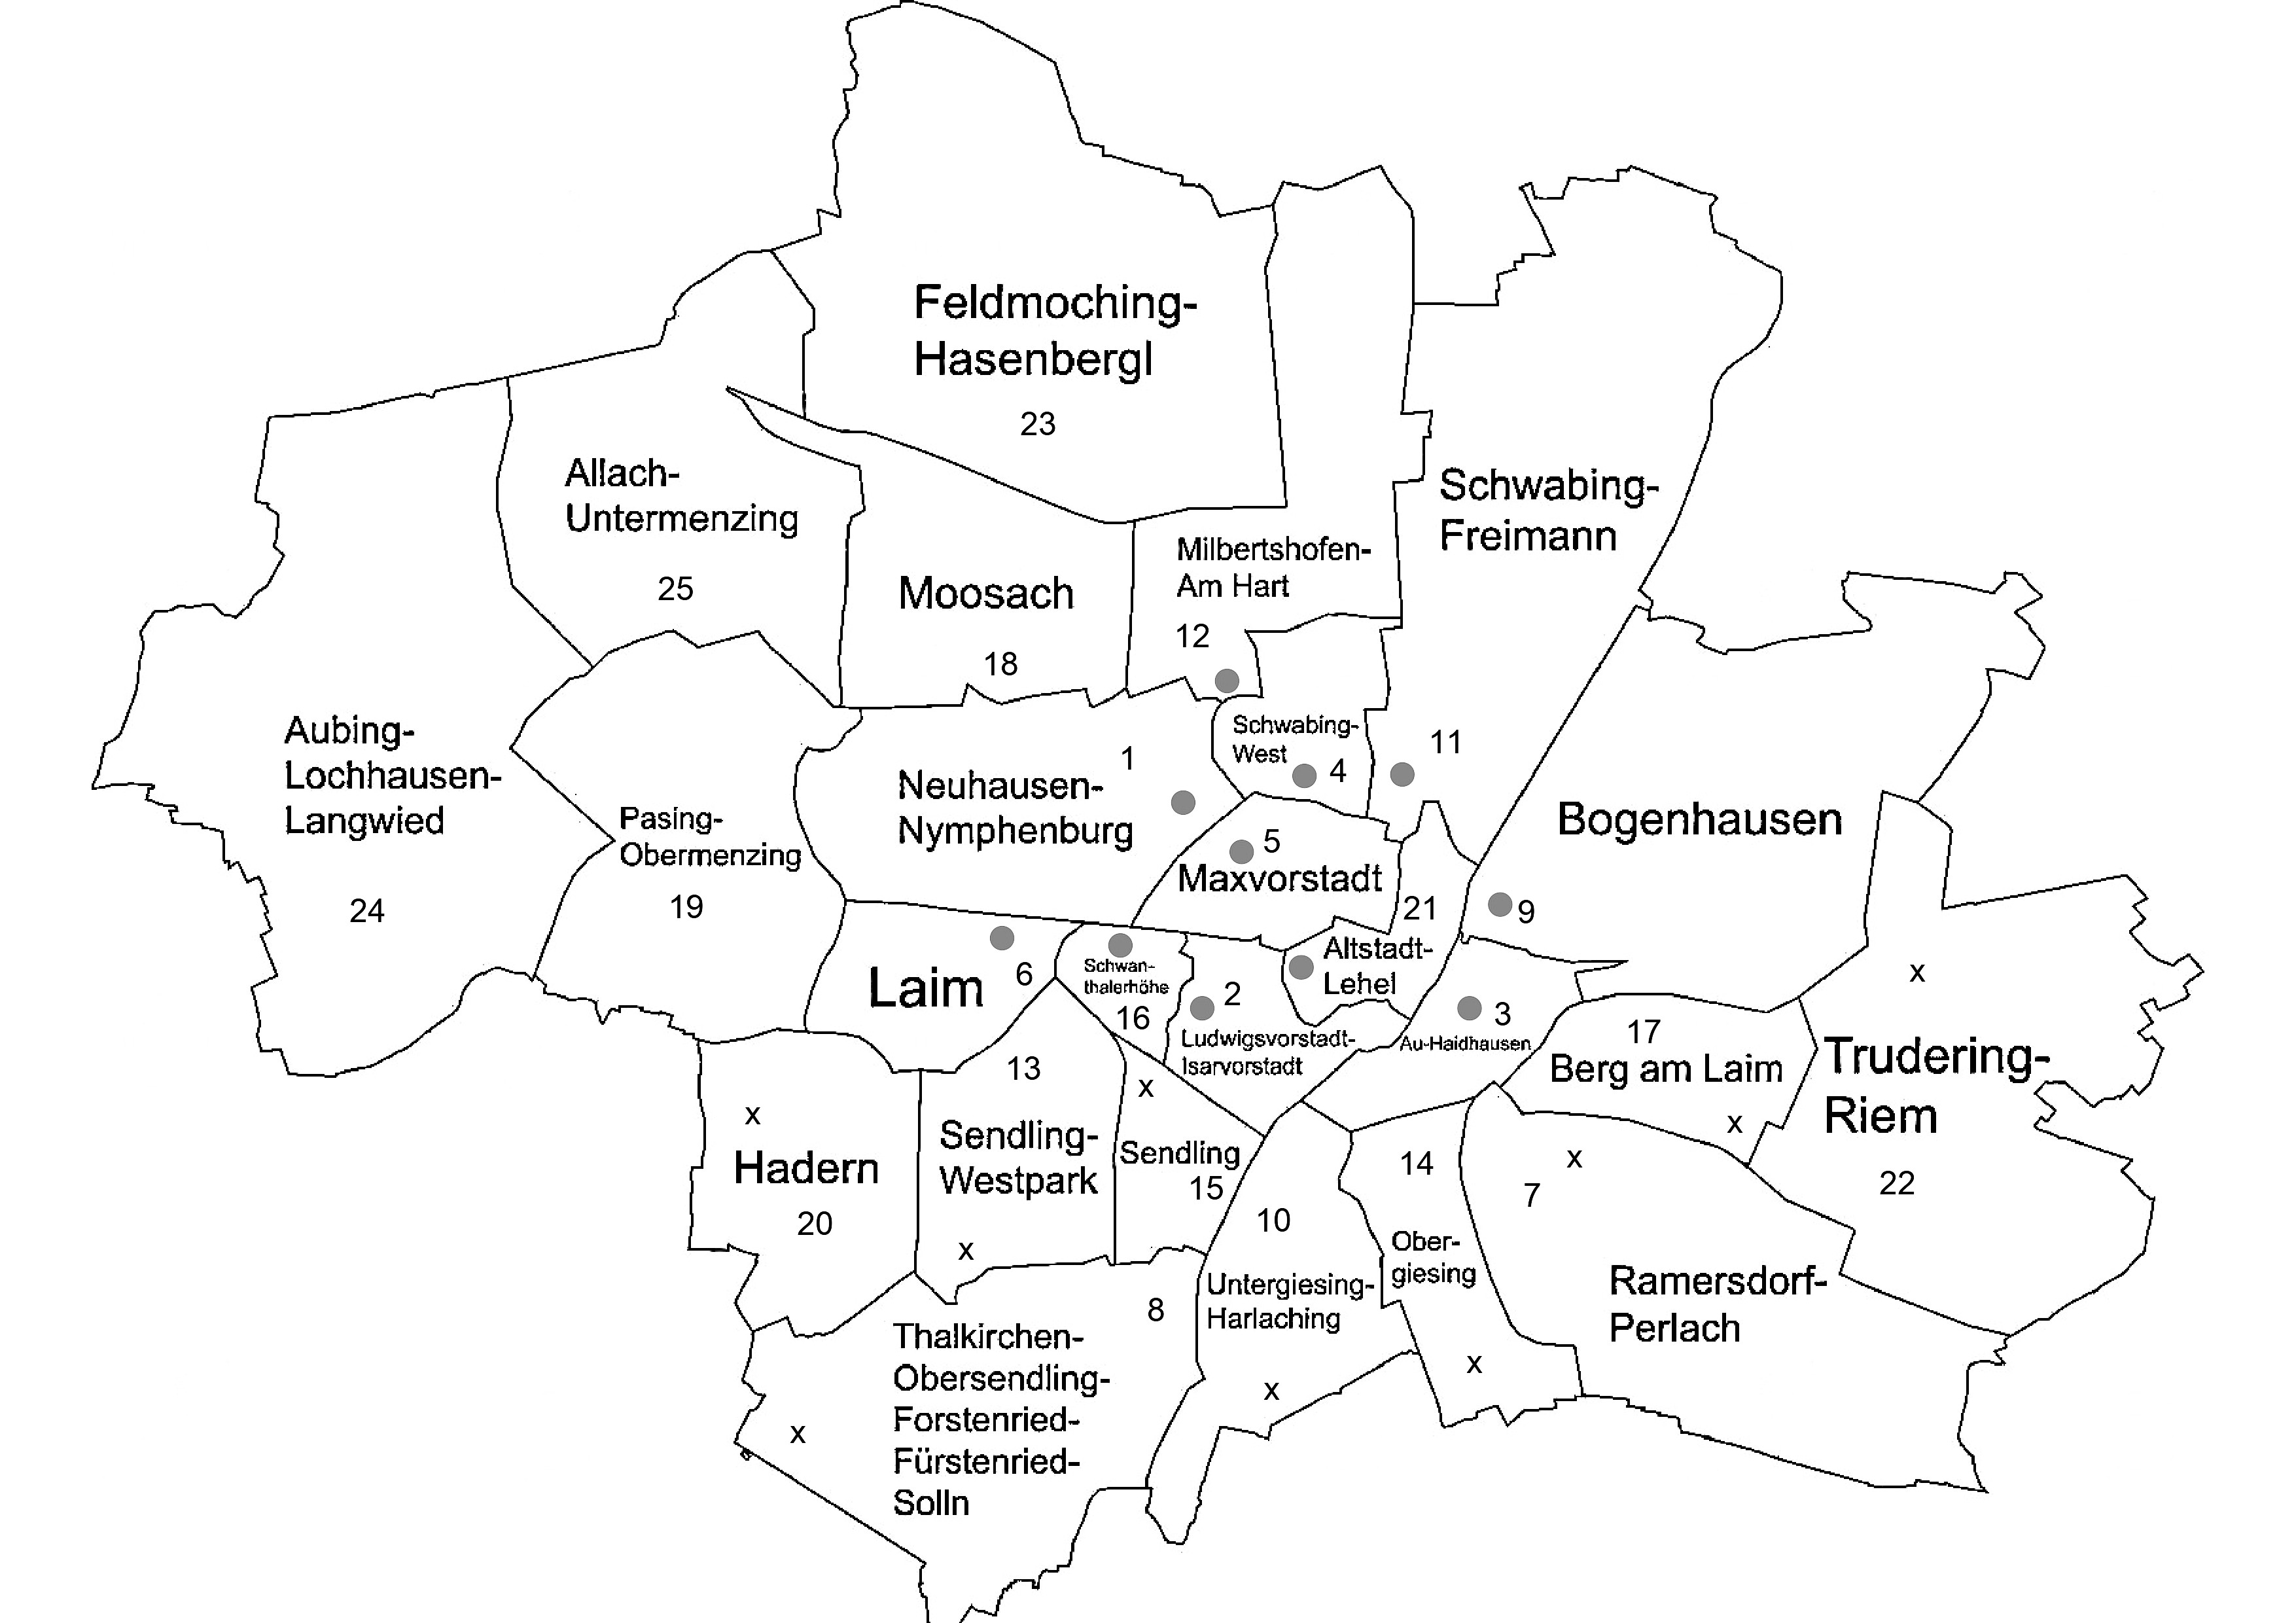
\includegraphics[width=0.5\textwidth]{munich_district.jpg}
	\end{figure}
	Once the districts were grouped into three areas, the following shows the distribution of houses across the areas.
			\begin{lstlisting}[language=R]
> table(data$district_group)

Area1 Area2 Area3 
1214   658   181 
	\end{lstlisting}
	\item Next, the variable \lstinline[language=R]|rooms|, which indicates the number of rooms in each house and only takes values from 1 to 6, was converted into a factor and treated as a categorical variable. The variable \lstinline[language=R]|location| is an ordered factor by default, so I converted it into a regular (unordered) factor to ensure compatibility with the modeling functions.
\begin{lstlisting}[language=R]
> data$rooms <- as.factor(data$rooms)
> data$location <- as.factor(as.character(data$location))
\end{lstlisting}
\item Now, only two continuous variables remain: \lstinline[language=R]|rent| and \lstinline[language=R]|area|. To model the data under the Multinomial distribution, I applied a discretization method to convert these variables into discrete ones, aiming to preserve as much information as possible. Specifically, the discretization technique used is called information-preserving discretization, also known as the \lstinline[language=R]|Hartemink| method. The details of this transformation are presented in the code file. For the sake of brevity, the method itself will not be discussed in this report. 

The function that performs this task from the package \lstinline[language=R]|bnlearn| directly transforms the two mentioned continuous variables into discrete ones, without creating new variables. The \lstinline[language=R]|rent| and \lstinline[language=R]|area| variables have now been transformed into discrete variables, each divided into a set of intervals.
\begin{lstlisting}[language=R]
> table(data_disc$rent)

[77.31,406.132] (406.132,687.072] (687.072,1789.55] 
582               923               548 
> table(data_disc$area)

[17,44]  (44,78] (78,185] 
307     1086      660 
\end{lstlisting}
The dataset after applying all the transformations described above is named \lstinline[language=R]|data_disc|, and its structure is as follows:
\begin{lstlisting}[language=R]
> str(data_disc)
'data.frame':	2053 obs. of  11 variables:
$ rent          : Factor w/ 3 levels "[77.31,406.132]",..: 3 3 2 2 3 3 1 2 2 1 ...
$ area          : Factor w/ 3 levels "[17,44]","(44,78]",..: 2 2 2 2 3 3 2 3 2 2 ...
$ rooms         : Factor w/ 6 levels "1","2","3","4",..: 2 2 3 3 4 4 2 3 1 3 ...
$ bathextra     : Factor w/ 2 levels "no","yes": 1 1 1 2 2 1 2 1 1 1 ...
$ bathtile      : Factor w/ 2 levels "yes","no": 1 1 1 1 1 1 1 1 1 1 ...
$ cheating      : Factor w/ 2 levels "yes","no": 1 1 1 1 1 1 1 1 1 1 ...
$ location      : Factor w/ 3 levels "good","normal",..: 1 1 1 2 1 2 2 2 2 2 ...
$ upkitchen     : Factor w/ 2 levels "no","yes": 1 1 1 1 2 1 1 1 1 1 ...
$ wwater        : Factor w/ 2 levels "yes","no": 1 1 1 1 1 1 1 1 1 1 ...
$ year_group    : Factor w/ 4 levels "1918-1959","1960-1969",..: 1 4 1 3 4 3 1 1 1 1 ...
$ district_group: Factor w/ 3 levels "Area1","Area2",..: 1 1 1 2 2 2 2 2 2 2 ...
\end{lstlisting}
\end{itemize}
\subsection*{Model Learning}
The detailed implementation for learning models from the data and selecting the most appropriate one can be found in the accompanying R code file. Additionally, understanding the modeling process requires background knowledge in topics related to Directed Graphical Models, such as learning methods, model learning algorithms, and more. A full discussion of these topics is beyond the scope of this report. Therefore, I will only present the final result.
For a deeper understanding of Directed Graphical Models, one may refer to the book: \textbf{\href{https://www.bnlearn.com/book-crc-2ed/}{Bayesian Networks With Examples in R}}.\\

After the model learning process and the selection of the most appropriate model, we arrive at the following result:
\begin{figure}[H]
	\centering 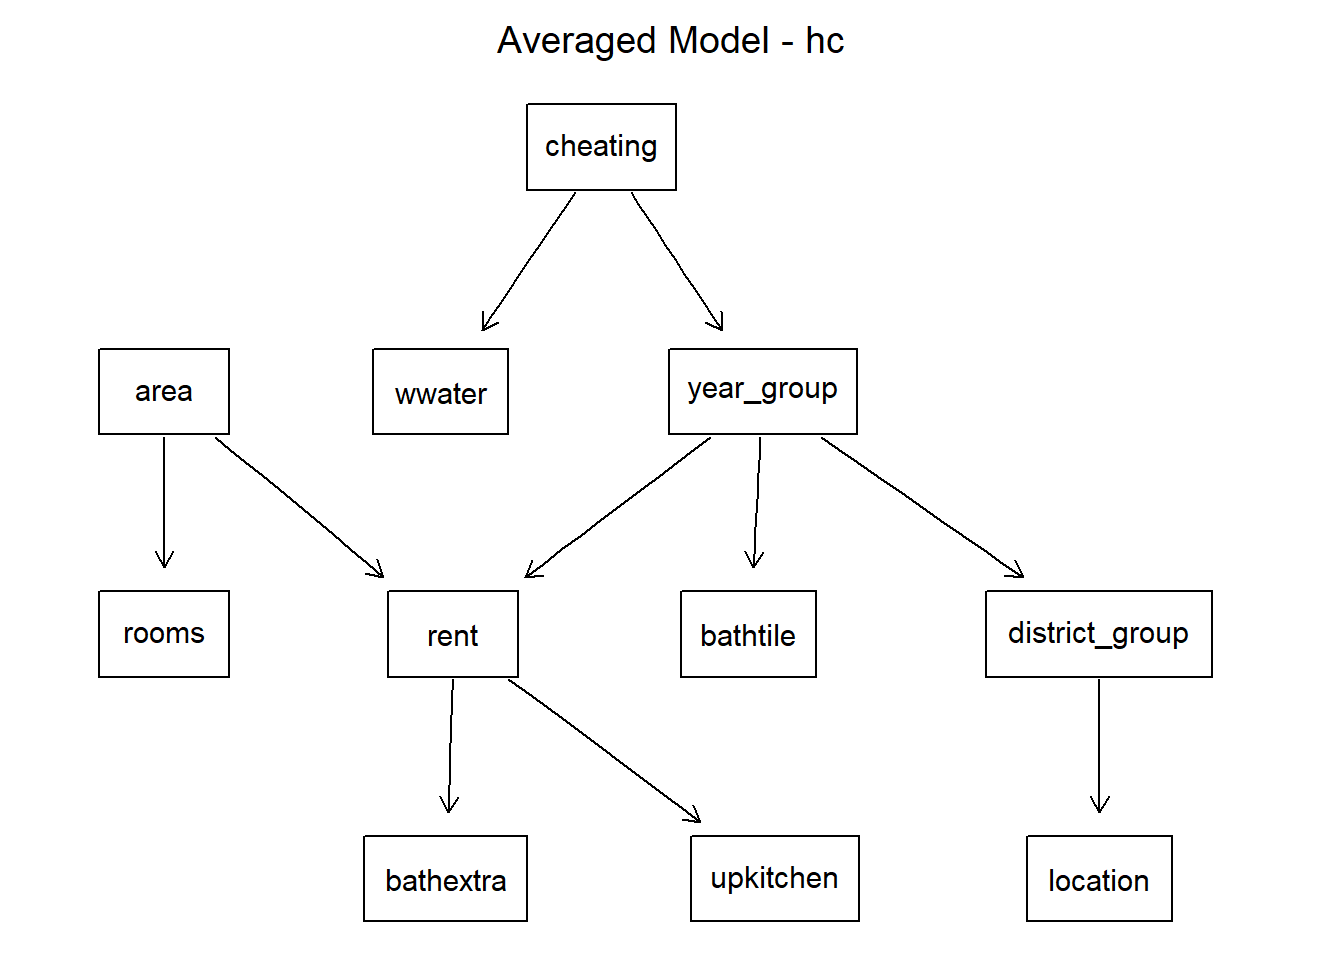
\includegraphics[width=0.6\textwidth]{unnamed-chunk-30-2.png}
\end{figure}
\section*{Inference and Querying}
\newpage

\end{document}